\documentclass[border=4pt]{standalone}
\usepackage{fontspec}
\usepackage{amsmath}
\usepackage{unicode-math}
\setmainfont{Latin Modern Roman}
\setmathfont{Latin Modern Math}
\usepackage{pgfplots}
\usepackage{pgfplotstable}
\pgfplotsset{compat=1.18}
\usepackage{tkz-euclide}
\usetikzlibrary{arrows.meta,calc,angles,quotes,patterns,3d,backgrounds}
\definecolor{ink}{HTML}{123428}
\definecolor{asy}{HTML}{475569}
\definecolor{mint}{HTML}{86e0bd}
\tikzset{asym/.style={asy, line width=0.9pt, dash pattern=on 5pt off 3.5pt},
         guide/.style={gray!70, line width=0.6pt, densely dotted},
         dot/.style={circle, inner sep=0pt, minimum size=5pt, draw=white, line width=0.5pt},
         odot/.style={circle, inner sep=0pt, minimum size=5.5pt, fill=white, line width=1pt},
         lab/.style={font=\footnotesize, inner sep=1.5pt, text=ink}}
\begin{document}
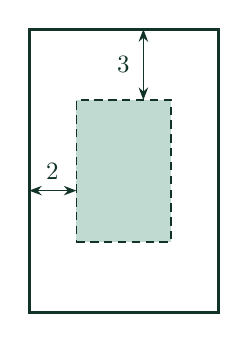
\begin{tikzpicture}
\draw[ink, line width=1.1pt] (0.000,0.000) -- (2.400,0.000) -- (2.400,3.600) -- (0.000,3.600) -- cycle;
\fill[color={rgb,255:red,4;green,107;blue,77}, opacity=0.25] (0.600,0.900) rectangle (1.800,2.700);
\draw[ink, line width=0.6pt, dash pattern=on 3pt off 2pt] (0.600,0.900) -- (1.800,0.900) -- (1.800,2.700) -- (0.600,2.700) -- cycle;
\node[font=\small, text=ink, inner sep=0.5pt] at (1.200,3.150) {$3$};
\node[font=\small, text=ink, inner sep=0.5pt] at (0.300,1.800) {$2$};
\draw[ink, line width=0.5pt, {Stealth[length=1.6mm]}-{Stealth[length=1.6mm]}] (1.450,2.700) -- (1.450,3.600);
\draw[ink, line width=0.5pt, {Stealth[length=1.6mm]}-{Stealth[length=1.6mm]}] (0.000,1.550) -- (0.600,1.550);
\end{tikzpicture}
\end{document}
